\chapter{2006 North American Monsoon Case Study} \label{ch:2006}

\ifpdf
    \graphicspath{{Chapter_2006/figures/PNG/}{Chapter_2006/figures/PDF/}{Chapter_2006/}}
\else
    \graphicspath{{Chapter_2006/figures/EPS/}{Chapter_2006/}}
\fi

Upper tropospheric ozone (O$_3$) has significant impacts on the radiative and chemical budgets of
the atmosphere \citep{Kiehl:1999uq}. The global tropospheric ozone burden has seen an
increase of 71--130~Tg since the preindustrial period, with much of the uncertainties
coming from the estimation of preindustrial emission scenarios for anthropogenic, biomass
burning, and lightning sources \citep[][and references therein]{Lamarque:2005gb}. The
radiative forcing resulting from this increase depends strongly on the vertical distribution and
is the most sensitive near the tropopause \citep{Lacis:1990fk}.

Previous studies have identified ozone enhancements, associated with monsoons, above North America
\citep[][and references therein]{Li:2005ss,Cooper:2009nx}, Asia \citep{Park:2007bh,Worden:2009ve},
and equatorial Africa \citep{Bouarar:2011ly} during summers in the upper troposphere (UT).
\citet{Cooper:2007cr} calculated an ozone enhancement of 29--52~ppbv between 10--11~km
above Huntsville, Alabama. This observed upper tropospheric ozone enhancement has
been linked to the North American Monsoon anticyclonic circulation, which traps ozone
precursors that subsequently enhance ozone production \citep{Li:2005ss}. \citet{Cooper:2009nx}
suggested that more than 80\% of the upper tropospheric NO$_\mathrm{x}$ within the enhancement
is due to lightning, and that it is responsible for 25--30~ppbv ozone at 250~hPa. Furthermore,
it has been estimated that the ozone enhancement generates a positive radiative forcing of about
0.50~W\,m$^{-2}$ \citep{Cooper:2007cr,Choi:2009bh}.

The primary goal of this study is to understand the causes of the summertime UT ozone enhancement by
using model diagnostics. To do this, regional-scale model simulations are performed to represent
the 2006 North American Monsoon. The control simulation is evaluated with multiple data sources to
show the contribution of boundary layer air (BL), stratospheric air (ST), and air from outside the model
domain (boundary condition, BC) to the O$_3$ enhancement.

\section{Model Description}\label{sect:setup}

The case study simulation is performed using the Weather Research and Forecasting model
\citep{Skamarock:2008xx} with Chemistry \citep[WRF-Chem;][]{Grell:2005fv} version 3.4.1
over July and August of 2006. The model is configured with a horizontal grid spacing of 36~km
on a Lambert conformal projection centered over the contiguous United Status (CONUS) as
shown in Figure~\ref{fig:domain}. Vertical levels are discretized into 51 levels of variable thicknesses
up to 10~hPa.

The meteorology is initialized and assimilated with data from the National Center for Environmental
Prediction (NCEP) Global Forecasting System (GFS) final (FNL) gridded analysis at 6-hr intervals
(00, 06, 12, 18~UTC). Nudging is performed for temperature and water vapor above the planetary
boundary layer (PBL). Nudging for horizontal winds is performed above model level 10 where the
pressure is $843\pm55$~hPa. Advection for moisture, chemicals, and passive tracer
variables are performed with positive-definite and monotonic limiters described in
\citet{Skamarock:2006wm, Wang:2009fk}.

To represent sub-grid scale convection, the Grell-3 (G3) convective parameterization, a modified version of the
\citet{Grell:2002bs} ensemble scheme, is used. The G3 scheme has 144 ($=3\times3\times16$) dynamic control and
static control/feedback closures with varying parameters. Though, subsidence over neighboring grid has been
disabled due to grid size of the current simulation. In addition, shallow convection is
enabled to permit ventilation of BL air by weak convection.
Cloud microphysics is represented by the \citet{Thompson:2008vn}
scheme. Shortwave
radiative transfer is represented with the Goddard two-stream method \citep{Chou:1998kx}.
Longwave radiative transfer uses the
Rapid Radiative Transfer Model (RRTM) \citep{Mlawer:1997vn}. The planetary boundary layer (PBL)
processes are parameterized with the NOAH land surface model \citep{Chen:2001ys} and the
Yonsei University (YSU) scheme \citep{Hong:2006fk}.

The chemical mechanism used in this study is the Regional Acid Deposition Model version 2
(RADM2) \citep{Stockwell:1990ez} compiled with a ``WRF-conformed'' version of the Kinetic
Preprocessor (KPP) \citep{Sandu:2006jl}. No aerosol is included in the simulation. Photolysis
rates are calculated using the fast Tropospheric Ultraviolet-Visible (FTUV) scheme \citep{Tie:2003ve}.
Chemical initial and boundary conditions are obtained from the Model for OZone and Related
chemical Tracers (MOZART-4) global chemistry model \citep{Emmons:2010fk}.

Anthropogenic emissions are prescribed using the 2005 National Emission Inventory (NEI05) from the
Environmental Protection Agency (EPA) and is reset everyday at 06~UTC, or 11:00 pm to 2:00 am
local time, to allow switching between weekdays (Monday -- Friday), Saturday, and Sunday
emissions. Biogenic emissions are parameterized using the Model for Emissions of Gases and Aerosols
from Nature (MEGAN2) \citep{Guenther:2006kl}. MEGAN2 uses a combination of climatological leaf area
index~(LAI), vegetation speciation, predicted model temperature, and predicted model solar radiation
to compute the biogenic VOC emissions consistent with the model meteorological state.

Lightning-generated NO$_\mathrm{x}$ emission is parameterized using a modified \citet{Price:1992wb}
method based on cloud-top height, which is determined from the G3 convective scheme's level of neutral buoyancy 
(LNB) adjusted by $-2$~km \citep{Wong:2013vn}, and scaled down by a factor of 10 ($\times0.1$) to match the observed total
flash count estimated from the cloud-to-ground (CG) records of the National Lightning Detection
Network (NLDN) \citep{Cummins:2009aa} and a crude estimate of the CG-fraction from the
\citet{Boccippio:2001ys} climatology. The NO emission is set to 350~moles per flash, consistent
with \citet{Barth:2012qf}, and is placed vertically following the \citet{Ott:2010lo} distributions.

Three passive tracers are released from the lateral boundary (BC), planetary boundary layer (PBL), and
the stratosphere (ST). The magnitudes of the tracers are reset to $1.0$ at their respective sources for every
time step. However, due to overlapping of the lateral boundaries and either PBL or ST, it is possible that
a grid may simultaneously contains BC tracer value of $1.0$ and PBL or ST value of $1.0$. Thus, the
summation of the three tracer values is not constrained to one. Consequently, the absolute values of
A lightning NO$_\mathrm{x}$ (LNO$_\mathrm{x}$) tracer is also emitted with
LNO$_\mathrm{x}$ emission. All four tracers also have a decaying twin with a lifetime of 24~hours.
Each decaying twin is reduced at each time step by $q/\tau$ where $q$ denotes the tracer mixing ratio
and $\tau$ is the loss rate. The effective age of air is then computed as $-\tau\ln\overline{Q}^{V,t}/\overline{Q'}^{V,t}$,
where $\overline{Q}^{V,t}$ is the passive tracer value and $\overline{Q'}^{V,t}$ is the decaying tracer value
integrated over space and time, to allow simple estimates of the time since the trace has left its source region.
These tracers are then allowed to be transported by advection, convective transport, and mixing 

%Conceptualize the tendency calculation of a scalar $S$ from time step $t$ to $t+1$ as follow:
%\begin{equation}\label{eqn:fulltendency}
%S^{(t+1)}-S^{(t)} = (\Delta_{chem}+\Delta_{conv}+\Delta_{vmix}+
%\mathbf{v}\cdot\nabla+w\delta_z)S^{(t)}\delta t + E_S^{(t)}+LS^{(t)}
%\end{equation}
%where the $\Delta$'s are the time-stepping operators for chemistry, convective transport, and vertical
%mixing, $\mathbf{v}$ is the horizontal wind vector, and $w$ is the vertical wind. $E_S^{(t)}$ and
%$LS^{(t)}$ are the emission and loss terms. Then, we may accumulate at every single time step for
%a specific process $p$ to obtain the total tendency $T$ for a scalar $S$ due to the said process up
%to time $t$ from initialization:
%\begin{equation}\label{eqn:tendency}
%T_p^{(t)}=\sum_{\tau=0}^{t-1}\Delta_pS^{(\tau)}\delta\tau
%\end{equation}
%All individual processes include nonlinear terms associated with the respective solver, and thus
%no information is loss during the accumulation process. Therefore, if
%$\langle E_S^{(\tau)}+LS^{(\tau)}\rangle_{\tau<t}=0$,
%we may expect $\sum_{p\in\mathcal{P}}T_p^{(t)}\equiv S^{(t)}-S^{(0)}$ to hold in the upper troposphere
%for the first five processes $\mathcal{P}$ in Equation~\ref{eqn:fulltendency} with the exception
%of NO, for which $E_S^{(t)}$ may not be zero.

\section{General results and Evaluations}\label{sect:results}

\subsection{Meteorology}\label{sect:val/met}

The influence of meteorology on chemistry is of significant importance for the formation of
the North American Monsoon ozone enhancement \citep{Li:2005ss,Cooper:2007cr,Barth:2012qf}.
In particular, convection has been shown to detrain boundary layer (BL) air, which has relatively low
ozone mixing ratios (compared to the upper tropospheric background values) yet is rich in ozone
precursors, into the upper troposphere, thus perturbing UT ozone distributions
\citep{Dickerson:1987hc,Kar:2004jl,Weinstock:2007yj}. Moreover, thunderstorms generate
NO$_\mathrm{x}$ from lightning, providing the means to accelerate the ozone production
in the convective outflow by supplementing to the NO$_\mathrm{x}$-poor BL air.
Because of the importance of convection on upper tropospheric ozone, we evaluate the
model-predicted precipitation and lightning flash rate with observations.

\subsubsection{Precipitation}

While precipitation is not a good measurement of the immediate convective strength, the
accuracy and availability of information from the National Weather Service (NWS) Advanced
Hydrological Prediction Service (AHPS) allows continuous evaluation of the model's
prediction. The data product used here is the daily precipitation product from NWS AHPS,
a national mosaic product using the combined data from 12 River Forecast Centers (RFCs).

A comparison of the simulated precipitation amount by WRF and
the observed precipitation from NWS AHPS during July and August of 2006 is shown in Figure~\ref{fig:precip_sd}.
WRF is producing a comparable spatial distribution to NWS but with a high bias at the
Arkansas/Texas border and a low bias over Tennessee and Kentucky. Another low bias
is located in North Carolina east of the Blue Ridge Mountains. The simulated coastal
rainfall north of the Gulf of Mexico is also generally lower than observed except for regions
near Houston, TX. The simulated bulk convective fraction is relatively
high, with more than 90\% of the precipitation coming from convective parameterization
over the majority of CONUS.

The WRF-predicted area mean precipitation amount of 71~mm during August for the analysis
region shown in Figure~\ref{fig:domain} is 14\% less than the 82~mm reported by the NWS
(Figure~\ref{fig:precip_ts}). This
error in precipitation is caused by under-prediction in the frequency of heavy precipitation events above
15~mm/day (Figure~\ref{fig:precip_ts}{\bf b}). A possible cause is that weak convective events
are over-predicted, thus reducing the availability of moisture and latent heat for heavier
events.

\subsubsection{Lightning}

Although the lightning flash rate was extensively evaluated by \citet{Wong:2013vn}, it
must be compared with observations for this case study because the precipitation distribution
differs from the model results reported by \citet{Wong:2013vn}.
We use Vaisala U.S. NLDN data for our evaluation of lightning flash
rates. The network provides continuous multiyear CONUS coverage of $>90\%$ of all CG
flashes with ongoing network-wide upgrades since 1984 \citep{Orville:2002uq,Orville:2010uq}.
The frequency range at which the sensors operate allows detection of primarily CG flashes
and a small number of IC flashes. Low peak current strokes $<15$~kA are eliminated from
the data set due to potential misclassification. The median location accuracy is 250~m, which
is well within the model grid size used in this study and thus may be considered negligible.
Multiple strokes are aggregated into a single flash if they are within 1~second and no more
than 10~km apart.

Since NLDN reliably detects only CG flashes in 2006 and the current implementation of
WRF-Chem produces total flash counts without IC\,:\,CG partitioning, flash count outputs
from WRF are scaled by $1/4$, or an IC\,:\,CG ratio of 3-to-1, to account for a crude average
of the CG fraction in southeastern United States according to \citet{Boccippio:2001ys}.
Without tuning, the CG flash count estimation is over-predicted by an order of magnitude, and
After the scaling, model flash count, summed over the analysis region for the two months simulated,
is 7\% higher than that observed by NLDN.
While the magnitude of the integrated flash count is similar to the NLDN observations,
its distribution truncates prematurely at $\sim200$~flashes/grid/day (Figure 4b) and compensates 
the deficit with an overestimation of flashes below
100~flashes/grid/day. This early truncation is consistent with the findings discussed by
\citet{Wong:2013vn}.

\subsection{Ozone}\label{sect:val/o3}

Since the ozone enhancement occurs primarily above the southern United States, it is
useful to define a region of focus different from that used in the precipitation evaluation.
We define the ``anticyclone region'' based on the August mean geopotential height
($\overline Z_{300}$) at 300~hPa simulated by the model. The anticyclone region is determined
by columns with $\overline Z_{300}>9730$~m. While the anticyclonic circulation is not stationary, using
the mean circulation maximizes the duration during which characteristics of the ozone
enhancement can be captured.

Both the August mean 300~hPa ozone and geopotential heights are shown in
Figure~\ref{fig:o3_map}a. The
location of the ozone enhancement is consistent with that observed and simulated by
\citet{Cooper:2007cr}. The ability to position the enhancement only requires the correct
large-scale dynamical features, which are constrained by nudging to NCEP GFS reanalysis.
North of the jet stream, persistently high ozone
concentration is simulated due to stratospheric ozone. It is found that some of this
ozone is occasionally mixed across the jet in the continental outflow region (northeast
corner of the model domain) and is then circulated into the anticyclone.

A finger-shaped low-ozone structure of $\sim65$~ppbv between the 9650
and 9700~m isohypses over south-central California separates the ozone enhancement
core and the northern stratospheric ozone as the result of repeated
low-ozone episodes flowing from the subtropical Pacific via the southwest corner boundary condition
provided by the MOZART global model prediction. The occurrence and path of this feature is controlled
by the monsoonal circulation and creates the gradient in the monthly mean that
partially forms the shape of the ozone enhancement.

\subsubsection{Evaluation against TES retrievals}\label{sect:val/o3/tes}

% n = 4699, max grid = 16

To evaluate the simulated ozone, retrievals from the satellite-borne
Tropospheric Emission Spectrometer (TES) are used to provide spatial snapshots
along selected transects. TES is a high resolution infrared Fourier-transform
spectrometer with a spectral resolution of 0.06~cm$^{-1}$ \citep{Beer:2006fk}.
The data products used are of V004, all of which are special observations in
step-and-stare mode with footprints of 5.3~km$\times$8.3~km and 35~km gaps
between stares. Through comparisons with ozonesondes, an evaluation with
V002 showed that TES ozone had a 3--10~ppbv high bias in the troposphere,
but it is still able to pick up the general variability \citep{Nassar:2008mw}. TES
products have been used in numerous studies on tropospheric chemistry
\citep[e.g.][]{Hegarty:2010vn,Voulgarakis:2011fk}, convection and water budget
\citep[e.g.][]{Brown:2008zr,Risi:2010ys}, and air quality
\citep[e.g.][]{McMillan:2010kx,Wang:2011uq}.

We first compare the ozone mean profile (Figure~\ref{fig:o3_map}) against TES. To
do so, WRF-Chem 3-hourly output column vectors are selected for each TES retrieval
pixel during August (Figure~\ref{fig:o3_map}b), then the averaging kernel, as will be
described below, is applied (Figure~\ref{fig:o3_map}c). This can be compared to the
monthly average TES product at 300~hPa, gridded onto $2^\circ\times2^\circ$ grids (Figure~\ref{fig:o3_map}d)
each of which receives 0--16 pixels for a total of 4699 pixels within the simulation
domain. The subsampling and application of the averaging kernel introduced noises
that prevents clear identification of the ozone enhancement. Though a high bias
can still be discerned while the general spatial distribution is consistent with TES observations.

We then compare the ozone curtain profiles. Between July 15 and August 23, ten TES
transects are selected and compared to the WRF-Chem output of the corresponding
date at 18~UTC or 21~UTC, whichever is closer to the 30$^\circ$N-crossing
time~(Figure~\ref{fig:o3_transect}). These transects are selected because they either show
signs of upper tropospheric ozone enhancement, or intersect regions with 300~hPa
geopotential height greater than 9730~m  while passing over the United States.
To compare model O$_3$ to TES profiles, the model profiles are transformed in
the same way as the satellite data. Let $\mathbf{x}_{\mathrm{WRF}}$ be the log of the ozone column
vector extracted from WRF-Chem and interpolated onto TES pressure levels, then the
averaging kernel is applied as follows:
	\begin{equation}\label{eqn:TES-AK}
		\mathbf{x}_{\mathrm{WRF}}^{\mathrm{TES}} = \mathbf{x_a} +
		\mathbf{A}\left(\mathbf{x}_{\mathrm{WRF}}-\mathbf{x_a}\right)
	\end{equation}
where $\mathbf{x_a}$ is the a priori constraint, $\mathbf{A}$ is the averaging kernel,
and $\mathbf{x}_{\mathrm{WRF}}^{\mathrm{TES}}$ is how TES would have observed the
WRF-Chem ozone column. Furthermore, columns with potential problems are filtered
out using the master quality assurance flag, the C-curve flag to remove retrievals with
anomalously high surface ozone \citep{Zhang:2010fk}, and the criteria that
$trace(\mathbf{A})>4.0$ to ensure sufficient degrees of freedom.

Figure~\ref{fig:o3_transect} shows the comparisons of model outputs and satellite retrievals along TES transects.
Qualitatively, the heights of the 100~ppbv ozone isopleths are well simulated north of
30$^\circ$N. South of 30$^\circ$N, upper tropospheric ozone is often over predicted.
These over-predictions occur either within Mexico, where the terrain of the Sierra Madre
triggers frequent large-scale thunderstorms, or the Gulf of Mexico, where LNO$_{\mathrm{x}}$
marine emission is unconstrained due to lack of observations. For example, transect 4911 (Aug 23, Figure~\ref{fig:o3_transect}j)
is able to capture the ozone enhancement between 28--47$^\circ$N, followed by a
ridge-like low ozone structure at 40$^\circ$N attributable to a low-ozone air mass
transported from the subtropical Pacific. South of 28$^\circ$N, where the transect
was passing over the Gulf of Mexico, WRF-Chem is biased high with the 100~ppbv
ozone isopleth reaching 300~hPa while TES observed only 70--90~ppbv up to 150~hPa.
Similar high biases are also seen for transects 4837 (Aug 15, Fig~\ref{fig:o3_transect}d)
and 4900 (Aug 21, Figure~\ref{fig:o3_transect}i).

WRF-Chem simulates higher ozone than observed by
TES in the upper troposphere (150--300~hPa) between 25--40$^\circ$N (Figure~\ref{fig:o3_distr}). TES observed a mean ozone
mixing ratio of 100~ppbv with a standard deviation of 22~ppbv. In contrast, WRF-Chem
simulated $120\pm31$~ppbv. The larger standard deviation from WRF-Chem indicates that
the predicted upper tropospheric ozone is less well-mixed than observations suggest.
The mid-troposphere (300--450~hPa) frequency distributions are much more similar in both mean
and width, with $78\pm17$~ppbv and $82\pm19$~ppbv for WRF-Chem and TES
respectively.

The above evaluations against TES retrievals show that while ozone is overestimated in the upper
troposphere, the existence of the ozone enhancement and its location are well-simulated.
Some drawbacks of using TES are the results' dependencies on a priori constraints and sparse
temporal resolution.



\subsubsection{Evaluation against IONS-06}

To complement the evaluation against TES, we use ozonesonde
profiles taken during the INTEX-B Ozonesonde Network Study of 2006
\citep[IONS-06;][]{Thompson:2008rp}. During this campaign, 410 ozonesondes were
launched from 14 sites strategically positioned to represent major sources, sinks, and
pathways of tropospheric ozone in North America. These sondes used electrochemical
concentration cell (ECC) sensors that have precisions within $\pm$(5--10)\% in the
troposphere \citep{Smit:2007ta}. Between different models of the instruments,
measurement biases due to variation in potassium iodide sensing concentration may be
on the order of 2--3\% \citep{Smit:2007ta}. Data from this campaign and its predecessor,
IONS-04, have been used to support studies on continental tropospheric ozone
distributions \citep[e.g.][]{Cooper:2007cr}, inferring local ozone sources
\citep[e.g.][]{Thompson:2008rp}, and evaluations of air quality models
\citep[e.g.][]{Tarasick:2007dq} and satellite retrievals \citep[e.g.][]{Nassar:2008mw}.

Ozonesondes launched during August 2006 within the model domain are compared
to WRF-Chem ozone vertical profiles. As an example, comparison at Huntsville, Alabama
is shown in Figure~\ref{fig:huntsville}. Despite the prevalent over-prediction of ozone
concentration in the upper troposphere, the timing of the occurrences of upper
tropospheric ozone enhancement episodes corresponds well with ozonesonde
measurements. Specifically, termination of the first enhancement on August~11
followed by a drop in ozone throughout the entire column is seen in both WRF-Chem
results and the ozonesonde profiles. Similarly, the termination of the second
enhancement on August~23/24  is also simulated. These events are likely caused by
the synoptic movements of the enhancement controlled by dynamical features. Over
all North American sites within the model domain, we find that the simulated ozone
mixing ratios above 200~hPa is a factor of 2--3 higher, for which the reason will
be explained in the second part of this manuscript.

In conclusion, WRF-Chem is able to simulate an upper tropospheric ozone enhancement
that coincides with the ``anticyclone region'' defined earlier, but the ozone mixing ratios
are overestimated primarily in the upper troposphere. Despite the high bias,
spatiotemporal variabilities controlled by large-scale dynamics are observed at individual
locations affected by the ozone enhancement.

\subsection{Carbon Monoxide}\label{sect:val/co}

To understand the ozone bias, it is useful to examine its chemical precursors. Carbon
monoxide (CO) is widely used for tracking boundary layer air and pollutants
\citep[e.g.][]{Pan:2007sw,Weinstock:2007yj}. Emitted through incomplete
combustion, CO  is an excellent indicator for anthropogenic emission sources and
biomass burning. It is also produced chemically through OH oxidation of a wide range
of VOCs. Furthermore, its 2--3 month lifetime in the troposphere allows CO to be an
effective long-range tracer.

Figure~\ref{fig:co_map}a shows the August mean CO mixing ratio at 300~hPa. At the
center of the NAM circulation is a distinct CO maximum over northeastern Texas. This
feature may be the result of a combination of CO accumulating via the NAM circulation
and local convective detrainment of boundary layer air. Considering the Texas/Arkansas region
shows a high bias in convective activities (Sect.~\ref{sect:val/met}), this feature
should be weaker than shown. On the other hand, the high CO simulated over
Georgia and neighboring states may have been underestimated because of the
under-prediction in convection along the Blue Ridge Mountains. North of the
jet stream, anomalously high CO found near the tropopause is a result of transported from the
western domain boundary. This influx of CO can be linked to intercontinental transport
of widespread wild fires across the Siberian plateau during July. Between these two regions
of high CO is an air mass with low CO and low ozone transported from the
subtropical Pacific into the inner CONUS between the 9600 and 9700 isohypses.

\subsubsection{Evaluation against TES retrievals}

To evaluate the predicted CO, we compare WRF-Chem results
against TES CO products. The instrument characteristics of TES are already described
in Section~\ref{sect:val/o3}. The TES CO product has been evaluated against the
Measurements of Pollution in the Troposphere (MOPITT) satellite
retrievals~\citep{Luo:2007ly,Ho:2009lh} and aircraft
measurements~\citep{Luo:2007vn,Lopez:2008ys}. These studies found that TES CO products
show slightly lower column CO values compared to MOPITT and a $\pm10\%$ bias
relative to in-situ measurements. The primary contributions being smoothing errors
and the dependency on the a priori constraint used for TES retrieval. Except for instances
of poor spatiotemporal coincidences, correlation coefficients between in-situ measurements
and TES retrievals are between 0.61 and 0.92. Therefore, while retrieval values may
be biased, the relative variabilities of CO are expected to be realistic.

The TES CO product is often utilized in tandem with the TES ozone product.
\citet{Logan:2008uq} used these two products to investigate the impact of El Ni\~no
on tropospheric composition. Similarly, \citet{Voulgarakis:2011fk} used them to
investigate the global O$_3$-CO correlation. We compare WRF-Chem CO
to the TES CO product using the procedure outlined in Equation~\ref{eqn:TES-AK},
similar to the comparison done with ozone in the  previous section except for a
minimum degrees of freedom of 0.8 and without the C-curve flag.

Similar to ozone, the August model output has been subsampled and transformed
in Figure~\ref{fig:co_map} to compare with the gridded TES monthly average. The mixing
ratio value is seen substantially overestimated though spatial variability is captured.

Figure~\ref{fig:co_transect} shows the WRF-Chem
CO mapped onto Tthe ES transects along with TES CO products. WRF-Chem is
biased high in the mid-to-upper troposphere. There are three possible causes for a high
bias in CO. The first being an underestimation of the CO loss rate, governed by dry deposition
and chemical losses via CO + OH, which may be subsequently attributed to photolysis
as OH is primarily controlled by the photolysis rate $J(\mathrm{O}_3)$ to form O($^1$D). The second
possible cause is an overestimation of boundary layer air detrainment. Even though
precipitation has been under-predicted overall (Sect.~\ref{sect:val/met}), there is
substantial over-prediction in the frequencies of light precipitation events
$<15$~mm/day~(Figure~\ref{fig:precip_ts}b). Finally, the high bias may be due to the
application of the TES averaging kernel as the MOZART distribution, though not utilized within
the interior of the WRF-Chem simulation, also shows a high bias (Figure~\ref{fig:co_distr}).

While there is a high bias in the upper troposphere connected to convective transport
or loss rate, there is a low bias at northern latitudes within the lower-to-mid troposphere.
A source for these low biases is that the current simulation did not prescribe biomass
burning emission via wildfire events. Using the fire products from the Moderate
Resolution Imaging Spectroradiometer \citep[MODIS;][]{Justice:2002zr}, several
enhanced CO plumes in the TES transects can be identified as fire related. On July
16, transect 4534 (Figure~\ref{fig:co_transect}a) captured a wildfire at Soda Creek, WY
(43.5$^\circ$N, 110.2$^\circ$W). On August 15 and 17, multiple transects
(Figure~\ref{fig:co_transect}e--g) captured the downwind plumes of widespread fires from
Oregon as heightened CO signature between 46--53$^\circ$N. Finally, transect
4911 captured the plume from the Idaho fires on August 23 (Figure~\ref{fig:co_transect}j).
Excluding wildfire events, WRF-Chem is almost always biased high.

The CO frequency distributions from the WRF-Chem results and TES CO retrievals for data
between 25--40$^\circ$ are shown in Figure~\ref{fig:co_distr}. The computed
mean values for the upper tropospheric distributions are 85~ppbv and 68~ppbv for
WRF-Chem and TES respectively, and thus WRF-Chem is 26\% too high.
In the mid-troposphere, the mean mixing ratios are 100~ppbv and 81~ppbv , thus
WRF-Chem is 22\% higher.

\subsection{Nitrogen Oxides}\label{sect:val/nox}

To evaluate the model's output of NO$_{\mathrm{x}}$, we compare tropospheric NO$_2$
vertical column densities (VCDs) to retrievals from the Scanning Imaging Absorption
Spectrometer for Atmospheric Chartography (SCIAMACHY) instrument on board of the
Environmental Satellite (ENVISAT) \citep{Burrows:1995fk,Bovensmann:1999uq}. The
instrument measures scattered and reflected sunlight in the thermal IR spectral range,
providing sensitivity to trace gases in the troposphere such as NO$_2$ and HCHO. The
retrieval used in this study is developed at the Royal Netherlands Meteorological
Institute~(KNMI) and obtained via the Tropospheric Emission Monitoring Internet
Service~(TEMIS) project (http://www.temis.nl). The retrieval algorithm uses the Differential
Optical Absorption Spectroscopy~(DOAS) method and a data-assimilation technique,
which utilizes a chemistry-transport model~(CTM) with ECMWF operational analyses
meteorology to estimate the stratospheric portion of the retrieved column
\citep{Boersma:2004uq}. Evaluation of the TEMIS NO$_2$ product has been performed
by \citet{Lambert:2004aa} against NDSC data, showing bias up to
$3.5\times10^{15}$~molec~cm$^{-2}$. The differences between retrievals have been
attributed mostly to the tropospheric air mass factor \citep{vanderA:2010aa}, which has
a sensitivity to cloud fractions of up to 20\% \citep{Boersma:2004uq}.

For the comparison, each SCIAMACHY tropospheric VCD data point is associated with
a single WRF-Chem column determined by rounding the time of measurement to the
nearest model output time (3-hourly). Due to ENVISAT's orbit, all measurements are
taken between 15--21~UTC. Matched WRF-Chem NO$_2$ partial columns are then
accumulated using the tropospheric VCD averaging kernel for levels below the
tropopause index computed using the WMO tropopause definition and provided with the satellite product. Over 61 days,
$5.2\times10^5$ pixels were selected. An individual model grid receives anywhere between 0
to 15 pixels, which is less than 20 ($\approx$61 days/3 days per global survey) due
to rejected measurements.

Using this procedure, the frequency distributions of WRF-Chem and SCIAMACHY
NO$_2$ tropospheric VCDs are calculated (Figure~\ref{fig:scia_no2}a). While the
WRF-Chem distribution is lognormal with a background close to
$0.1\times10^{15}$~molec~cm$^{-2}$, the SCIAMACHY distribution is closer to a
normal distribution skewing towards the left with a negative tail. Negative values
in tropospheric column retrievals are permitted because of the retrieval process,
which involves estimating and subtracting the stratospheric NO$_2$ partial column.
Despite the differences in the distributions, the modes for both distributions are
$\sim0.5\times10^{15}$~molec~cm$^{-2}$, consisting mostly of data points from
the Pacific marine columns, Idaho/Montana, and Canada. Spatial distributions of
most regions are well-simulated with a high bias in regions with high flash
rates of $\sim2\times10^{15}$~molec~cm$^{-2}$, over a background of 0.5--1$\times 10^{15}$~molec~cm$^{-2}$,
which is within the potential range of retrieval biases.

\subsection{Evaluation summary}\label{sect:val/summary}

A case study simulation is performed using WRF-Chem with specific physics and
chemistry options described in Section~\ref{sect:setup} for the 2006 North American
Monsoon. We found that the model produces the following results compared to
various in situ or remote sensing observations:
\begin{enumerate}
\item Convective strength, proxied by precipitation, is generally distributed similar to observations, but
with an overall underestimation in integrated rainfall while overestimating at certain locations;
\item Lightning flash rate is estimated to be within the range of variability of the NLDN CG flash counts when using
a scaling factor of $0.1$ and an approximated bulk IC\,:\,CG ratio of 3\,:\,1;
\item Ozone is over-predicted by $\sim20\%$ in the upper troposphere but largely consistent
with TES retrievals in the mid-to-upper troposphere in terms of spatiotemporal and frequency distributions;
\item Carbon monoxide (CO) is also over-predicted compared to TES retrievals in the upper troposphere;
\item NO$_2$ VCDs are simulated within the range of retrieval uncertainties.
\end{enumerate}

\section{Tracer diagnostics}\label{sect:diag}

While the ozone enhancement occurs in the upper troposphere largely within the ``anticyclone
region,'' as previously defined as the columns with an August mean geopotential height of 9730~m
or greater, the air the comprises of the enhancement volume originates from various regions and
sources. Thus to reconcile the composition and air mass sourcing, we examine tracer-tracer
correlations and passive tracer diagnostics, as described in Section~\ref{sect:setup}.

\subsection{O$_3$-CO relation}\label{sect:diag/tracer}

The relationship between ozone and carbon monoxide ({CO}) has been
used to study the tropospheric-stratospheric transition in chemical regimes
\citep[e.g.][and references therein]{Pan:2007sw,Hegglin:2009fk}. Similarly,
such analysis may be applied to tropospheric data alone to identify contributions
from various pathways \citep[e.g.][]{Zhang:2006zr,Voulgarakis:2011fk,Cristofanelli:2013uq}.
In the troposphere, CO has a high volume mixing ratio (VMR) near the surface and low VMR in the upper
troposphere because of anthropogenic surface emissions. Ozone, on the other hand,
has high values near the tropopause because of transport from the stratosphere.
Together, the {O$_3$-CO} anti-correlation over a sufficiently expansive column
can expect to form an ``L''-shaped joint distribution.

Figure~\ref{fig:o3co} shows the joint-distributions at three separate pressure ranges
computed both inside ($\overline Z_{300}>9730$) and immediately
outside ($9710<\overline Z_{300}<9730$) the anticyclone north of 25$^\circ$N for
August between 15--21~UTC. Both distributions exhibit the expected ``L''-shaped
structure. The most frequency mixing ratios (modes) are near 55~ppbv~CO/70~ppbv~O$_3$ and 55~ppbv~CO/50~ppbv~O$_3$ for
upper troposphere and mid-troposphere, respectively, in both within and just outside the anticyclone.
However, the mode inside the anticyclone is 68~ppbv~CO/30~ppbv~O$_3$ while that
just outside of the anticyclone is 52~ppbv~CO/17~ppbv~O$_3$ for levels below 700~hPa
because of the large number of remote data points.
In addition, data points with both high CO and high O$_3$ (feature ``X'' in Figure~\ref{fig:o3co})
are more commonly found within the anticyclone in the upper troposphere and only
found within the mid-troposphere within the anticyclone, indicating that chemical
production in the mid-to-upper troposphere is indeed enhanced. Finally, there is
a relatively larger fraction of data points within the mid-troposphere with both low CO
and low O$_3$ outside the anticyclone (feature ``+'' in Figure~\ref{fig:o3co}), which
is comprised largely of air diluted by clean sources from the Pacific.

\subsection{Air mass tracers}\label{sect:diag/passive}

Air mass passive, i.e. non-reactive, tracers can be used to diagnose the contribution of different tropospheric
regions to the upper tropospheric anticyclone. Tracers released from the lateral
boundaries (BC), the boundary layer (BL), the stratosphere (ST), and with lightning
NO$_{\mathrm{x}}$ are shown in Figure~\ref{fig:tracer}. The impact of the NAM circulation is
clearly shown in the spatial distribution of the lateral boundary (BC) tracer
(Figure~\ref{fig:tracer}a). Within the anticyclone region ($\overline Z_{300}>$9730~m),
the air mass a mean of $97.6\pm0.3\%$ of BC tracer over August, but normalizes
to $86\pm2\%$ as a fraction of the total ($\equiv$BC+BL+ST). Taking into account
loss of characteristics over time, BC tracer value within the anticyclone may be substantially
reduced to no more than $1.2\pm1.8\%$ with the 1-day decaying tracer, compared to
$8.2\pm9.5\%$ immediately outside the anticyclone between 9710 and 9730~m.
Thus, the impact of air from the boundary
condition, e.g. clean subtropical Pacific air, on the ozone enhancement is minimal.

The lightning NO$_{\mathrm{x}}$ tracer (LT) also shows substantial localized
enhancement within the anticyclone (Figure~\ref{fig:tracer}g). The observed eastward
shift from the 9730~m contour can be explained by the overall higher lightning
flash rate in the southeastern United States. The maximum accumulated passive
LT tracer is 3~ppbv within the anticyclone.

On the other hand, the boundary layer (BL) tracer shows little correlation with
the shape or positioning of the anticyclone. Instead, the features of the tracer
at 300~hPa are dominated by the orographic influence from the Rocky Mountains
near 115$^\circ$W (Figure~\ref{fig:tracer}c). Similarly, the stratospheric (ST) tracer
shows negligible influence from the anticyclonic circulation except for the influx
of air with high ozone associated with mesoscale eddies in the region of strong
wind shear near the jet in the continental outflow region along the eastern seaboard.

The ``equivalent'' age of the tracer can be estimated based on the procedure described in Section~\ref{sect:setup}
Due to mixing by processes such as injection of fresh BL air by convective outflow,
the age values may not be interpreted literally. Alternatively, one may interpret
an air mass of a certain age as having the same expected characteristics as a
purely aging parcel of the same age. Both BC and LT ages show clear distinctions
across the anticyclone region boundary. The range of ages for the BC tracer within
the anticyclone is $4.7\pm0.8$~days, while the range immediately outside the anticyclone
between 9710~m and 9730~m is $3.0\pm1.0$~days. LT tracer age ranges from 10.9--21.8~hrs
within the anticyclone and 13.1--22.5~hrs just outside. Since the LT distribution is
heavily influenced by areas with high lightning flash frequency, young LT tracers
are expected and found  only within the eastern $\sim2/3$ of the anticyclone as
well as towards the outflow region. Similar to tracer values, neither BL nor ST tracer ages show
any differences across the anticyclone region boundary. BL and ST ages inside
the anticyclone are $3.8\pm0.6$~days and $5.3\pm1.1$~days respectively, while
the ages just outside the anticyclone are $4.1\pm0.7$~days for BL and $5.5\pm1.4$~days for ST.

\section{Discussion}\label{sect:disscusion}

The North American Monsoon upper tropospheric ozone enhancement has
been studied previously by \citet{Li:2005ss},
\citet{Cooper:2006dq,Cooper:2007cr,Cooper:2009nx}, and \citet{Barth:2012qf}.
Among these studies, \citet{Cooper:2007cr} and \citet{Barth:2012qf} also focused
on the 2006 North American Monsoon due to the stronger anticyclone
and availability of additional measurements from IONS-06. However, despite
being ``stronger,'' the circulation is often offset from the mean state and its center is
occasionally seen over California \citep{Barth:2012qf}. Therefore, despite the
ozone mean showing enhanced concentration over the southern United States, coinciding
with the mean monsoonal circulation, the instantaneous positions of the anticyclone are
often not correlated with the mean ozone enhancement seen in the Figure~\ref{fig:o3_map}.
Nonetheless, enhanced mean upper tropospheric ozone over the southern United States
has real consequence on the radiative budget \citep{Cooper:2007cr}.

Despite overestimation of ozone concentration, the positioning of the mean ozone
enhancement is largely consistent with \citet{Cooper:2007cr}, which only
requires the simulated synoptic dynamics to be similar. Furthermore, both our simulations
show low ozone coming in from the Pacific, producing the sharp gradient that forms
the western edge of the mean ozone enhancement. Finally, enhanced lightning
NO$_{\mathrm{x}}$ is also found within the NAM circulation in both studies.

We found that boundary layer and stratospheric tracers concentrations
and ages in the upper troposphere within the anticyclone is not substantially different from
those outside the circulation. On the other hand, tracer diagnostics show that the mean lateral
boundary tracer age is about a day older inside the anticyclone. Thus, we hypothesize
that a driver for the apparent ozone enhancement is not that of internal accumulation of
convectively-detrained boundary layer ozone precursors, but rather the lack of
external factors such as dilution by clean air masses from the Pacific.

Moreover, despite LNO$_{\mathrm{x}}$ tracer being higher within the anticyclone, the
lower concentration on the western 1/3 over the Rocky Mountain indicate that the
primary driver for the tracer enhancement may not be the circulation, but rather the
coincidence of high flash rate regions, VOC emission sources \citep{Barth:2012qf}, and the lack of external
influence.

\section{Summary}\label{sect:summary}

Using the Weather Research and Forecasting model with Chemistry (WRF-Chem),
we have simulated the upper tropospheric ozone enhancement during the North
American Monsoon in 2006 and evaluated its sources of variability using tracer
diagnostics computed within the model. Despite overestimation of upper tropospheric
ozone and carbon monoxide, evaluated against TES satellite retrievals, we found that the positioning
of the mean ozone enhancement is consistent with that found by \citet{Cooper:2007cr}.
Furthermore, with a tuned lightning parameterization, we found that our 
NO$_2$ vertical column density is also within retrieval bias of the SCIAMACHY
product used.

By examining the O$_3$-CO relation, not only did we find enhanced chemical production
within the anticyclone, but heightened presence of air with both low O$_3$ and low CO
immediately outside the anticyclone at the mid-to-upper troposphere levels, indicating the existence of a
source for dilution outside. Conversely, clean air from the southwestern model
boundary is steered away from the mean circulation region, thus the absence of
dilution adjacent to diluted region partially contributed to the observed ``enhancement''
gradients.

Passive tracers computed along with the model simulation reveal that
contrary to previous studies \citep[e.g.][]{Li:2005ss,Cooper:2007cr,Barth:2012qf},
boundary layer sourced tracer and stratospheric sourced tracer are not simulated
to be accumulating within the North American Monsoon circulation. On the other
hand, it is shown that the air within the anticyclone lacks lateral boundary tracer,
which includes clean air from locations such as the Pacific that can cause significant
dilution outside. Thus, we hypothesize that the appearance of the ozone
enhancement is not due to accumulation of boundary layer precursors as
stated by \citet{Li:2005ss}. Instead, the lack of dilution is the primary cause. Finally,
consistent with \citet{Cooper:2007cr}, lightning NO$_{\mathrm{x}}$ tracer shows enhanced values
within the eastern-$2/3$ of the anticyclone, which subsequently enhances
chemical production. However, the occurrence of this tracer enhancement
can also be attributed to coincidence of regions with high flash rates instead
of simply due to dynamics.

In the next chapter, we shall examine further the dynamical and chemical
structure associated with the enhancement as well as the associated sensitivities
to lightning NO$_{\mathrm{x}}$ emission.

% Model domain
 \begin{figure}
 \noindent\includegraphics[width=20pc]{figures/domain.eps} % png available
 \caption{WRF-Chem model domain (red). Marked inner region (blue) is used for various analysis.}
 \label{fig:domain}
 \end{figure}

 % Precipitation validation (map)
 \begin{figure}
 \noindent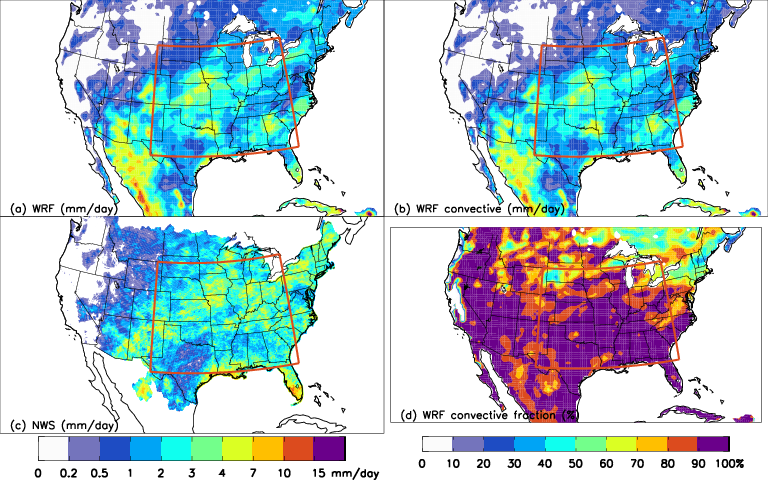
\includegraphics[width=40pc]{figures/precip_sd.png}
 \caption{(a) WRF-simulated total precipitation, (b) WRF-simulated convective precipitation, and
(c) total NWS AHPS precipitation in mm/day. (d) Parameterized fraction (\%) of model simulated
precipitation.}
 \label{fig:precip_sd}
 \end{figure}

% Precipitation validation (time series)
 \begin{figure}
 \noindent\includegraphics[width=20pc]{figures/precip_ts.eps} % png available
 \caption{(a) WRF and NWS daily area mean precipitation within the inner analysis region shown
in Figure~\ref{fig:domain} during August 2006. (b) Frequency distribution within the analysis region
with bin size 0.2~mm/day.}
 \label{fig:precip_ts}
 \end{figure}

% Lightning validation
 \begin{figure}
 \noindent\includegraphics[width=20pc]{figures/ltng_dist.eps} % png available
 \caption{(a) NLDN CG daily flash count ($\times10^4$) within the analysis region, with
WRF-simulated total flash count $\times1/4$ to account for CG fraction and $\times0.1$
to account for systematic bias. (b) Daily grid flash count frequency distributions from
NLDN and WRF with different scaling factors.}
 \label{fig:lightning}
 \end{figure}

% Ozone map
 \begin{figure}
 \noindent\includegraphics[width=40pc]{figures/o3/tes08_o3.png}
 \caption{(a) Simulated ozone (ppbv) and geopotential height (m) at 300~hPa averaged for August
2006. The 9730~m geopotential height contour indicates the ``anticyclone region'' used for
various analyses. (b) Ozone 3-hourly outputs sampled to all TES transects during August, and gridded
to $2^\circ\times2^\circ$ regular grids. (c) Previous panel with the TES averaging kernel applied.
(d) Gridded average of all August TES transects.}
 \label{fig:o3_map}
 \end{figure}

% TES-WRF ozone transect comparisons
 \begin{sidewaysfigure}
 \includegraphics[width=50pc]{figures/o3/transect_mosaic.pdf}
 \caption{First row for each panel is the WRF-Chem ozone profiles in ppbv mapped onto the TES
pressure coordinates after applying Eqn.~\ref{eqn:TES-AK}. Second row is the TES profile. Horizontal
dashed line indicates the 300~hPa level. Third row shows the TES transect and the 9730~m
geopotential contour at 300~hPa from WRF. Time indicated is the 30$^\circ$N-crossing time in UTC.}
 \label{fig:o3_transect}
 \end{sidewaysfigure}

% TES-WRF ozone freuency distribution comparisons
 \begin{figure}
 \noindent\includegraphics[width=20pc]{figures/o3/o3_teswrfhist.eps} % png available
 \caption{Normalized frequency distributions (\%/ppbv) of TES and WRF-Chem ozone mixing ratios
between (a) 150--300~hPa and (b) 300--450~hPa between 25--40$^\circ$N.}
 \label{fig:o3_distr}
 \end{figure}

% IONS-06 comparison
 \begin{figure}
 \noindent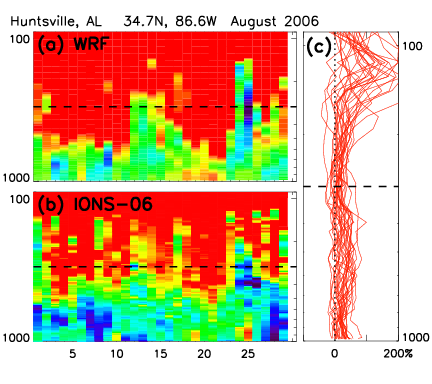
\includegraphics[width=20pc]{figures/o3/ions_huntsville.png} \\
 \noindent
\includegraphics[width=20pc]{figures/o3/o3_colorbar.png}
 \caption{WRF-Chem ozone vertical profiles in ppbv during August IONS-06 ozonesonde launches at
Huntsville, Alabama and the relative bias against the measured ozone mixing ratios. Horizontal
dashed lines indicate the 300~hPa levels in each panel.}
 \label{fig:huntsville}
 \end{figure}

% Carbon Monoxide map
 \begin{figure}
 \noindent\includegraphics[width=40pc]{figures/co/tes08_co.png}
 \caption{Same as Figure~\ref{fig:o3_map}, except for carbon monoxide.}
 \label{fig:co_map}
 \end{figure}

% TES-WRF CO transect comparisons
 \begin{sidewaysfigure}
 \includegraphics[width=50pc]{figures/co/transect_mosaic.pdf}
 \caption{Same as Figure~\ref{fig:o3_transect}, except for carbon monoxide.}
 \label{fig:co_transect}
 \end{sidewaysfigure}

% TES-WRF CO freuency distribution comparisons
 \begin{figure}
 \noindent\includegraphics[width=20pc]{figures/co/co_teswrfhist.eps} % png available
 \caption{Same as Figure~\ref{fig:o3_distr}, except for carbon monoxide and TES-adjusted
MOZART distributions are also provided for reference.}
 \label{fig:co_distr}
 \end{figure}

% SCIAMACHY NO2 validation
 \begin{figure}
 \noindent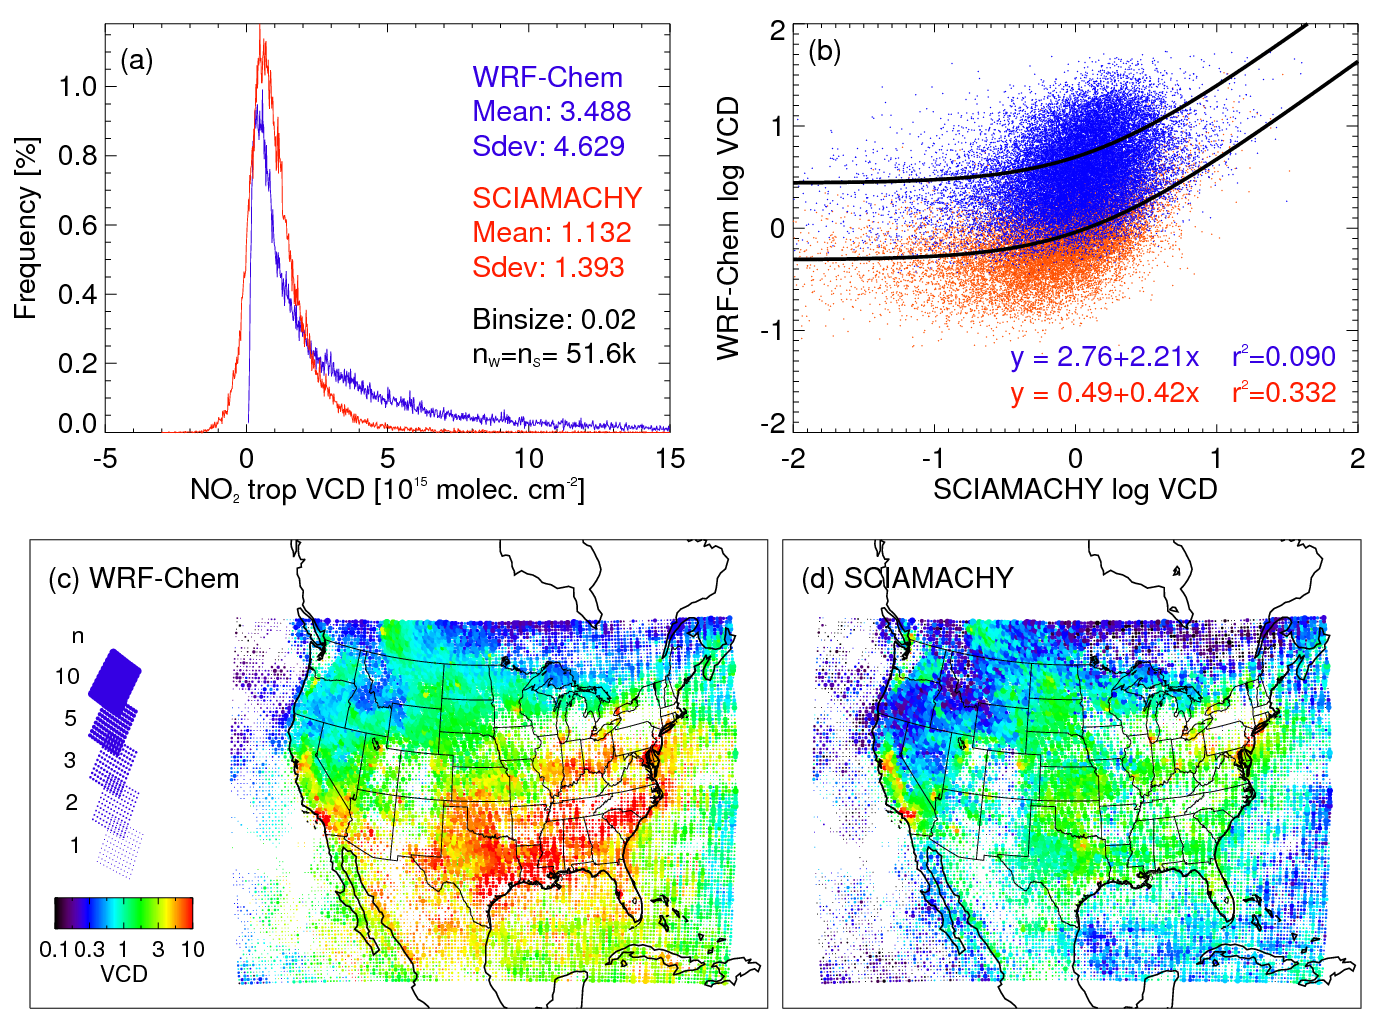
\includegraphics[width=40pc]{figures/scia_no2.png}
 \caption{(a) Frequency distributions of WRF-Chem and SCIAMACHY NO$_2$ tropospheric
VCDs in $10^{15}$~molec~cm$^{-2}$ during July and August 2006. A log-log plot of the
tropospheric VCDs and the corresponding minimized $\chi^2$ linear fit and correlation
coefficient $r^2$. (c) Mean WRF-Chem tropospheric VCDs in $10^{15}$~molec~cm$^{-2}$
with pixel density indicating the number of samples used (up to $n=15$ but saturates at
10) at each grid point. (d) Same as c, but for SCIAMACHY.}
 \label{fig:scia_no2}
 \end{figure}

% Tracer map
 \begin{figure}
	\noindent\includegraphics[width=20pc]{figures/o3co.eps} % png available
	\caption{O$_3$-CO joint-distributions (a) inside ($\overline{Z}_{300}>9730$~m)
	and (b) outside (9710~m$<\overline{Z}_{300}<$9730~m) the anticyclone region for
	the upper troposphere (100--300~hPa), lower troposphere ($>700$~hPa), and mid-troposphere (300--700~hPa).
	Contours are calculated in log-scale with 10 levels between $10^{-3}$ to $10^{-1}$~\%~ppbv$^{-2}$.
	Features ``X'' and ``+'' are used for discussions in Sect.~\ref{sect:diag}.}
 	\label{fig:o3co}
 \end{figure}

% Tracer map
 \begin{figure}
 \noindent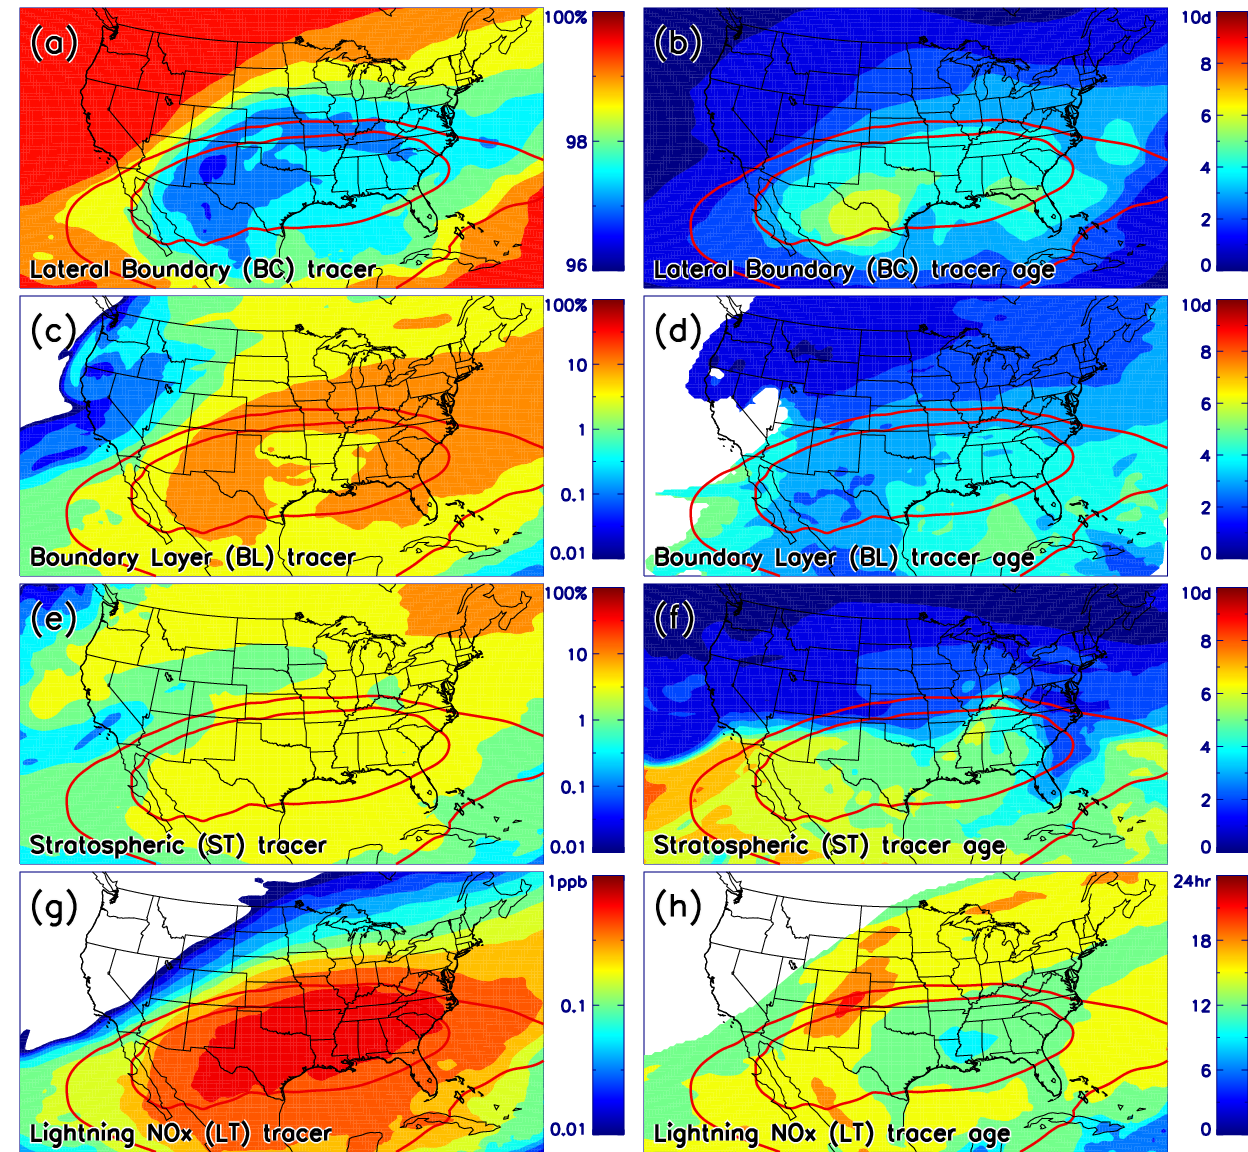
\includegraphics[width=40pc]{figures/tracer_maps.png}
 \caption{Passive tracer values (left column) and ages (right column) at 300~hPa averaged for August.
9710~m and 9730~m geopotential heights are also shown.}
 \label{fig:tracer}
 \end{figure}
